\documentclass[tikz, border=16pt]{standalone}
\usepackage{tikz}
\usetikzlibrary{arrows.meta, fit, backgrounds}

% ── Colour palette ─────────────────────────────────────────────────────────
\definecolor{clrInput}  {HTML}{4A90D9}
\definecolor{clrTool}   {HTML}{27AE60}
\definecolor{clrLLM}    {HTML}{E67E22}
\definecolor{clrCtrl}   {HTML}{8E44AD}
\definecolor{clrOutput} {HTML}{C0392B}
\definecolor{clrBg}     {HTML}{F7F9FC}
\definecolor{clrSub}    {HTML}{2C3E50}

% ── Styles ─────────────────────────────────────────────────────────────────
\tikzset{
  box/.style = {
    rectangle, rounded corners=4pt,
    minimum width=52mm, minimum height=9mm,
    text centered, font=\sffamily\small,
    draw, thick, text=white,
  },
  input/.style  = {box, fill=clrInput},
  tool/.style   = {box, fill=clrTool},
  llm/.style    = {box, fill=clrLLM},
  ctrl/.style   = {box, fill=clrCtrl},
  output/.style = {box, fill=clrOutput},
  panel/.style  = {
    rectangle, rounded corners=6pt,
    draw=clrSub, thick, dashed,
    fill=clrBg, fill opacity=0.55,
    inner sep=10pt,
  },
  arr/.style  = {-{Stealth[length=6pt]}, thick, color=clrSub},
  rarr/.style = {-{Stealth[length=6pt]}, thick, color=clrCtrl, dashed},
  lbl/.style  = {font=\sffamily\scriptsize\itshape, text=clrSub, midway},
  % legend entry box (smaller)
  legbox/.style = {box, minimum width=10mm, minimum height=7mm,
                   font=\sffamily\scriptsize},
}

% ── Layout ─────────────────────────────────────────────────────────────────
%   Left  column  x = 0    : INPUT → hdr → WHILE → get_item   (top 4 nodes)
%                            legend                              (lower left)
%   Right column  x = 9.2  : sub-workflow  dl … paper_reducer
%                            then: list_append → brief_writer → COMMIT
%
%   Horizontal CALL arrow aligns  gurl  ↔  dl      (y = -6.0)
%   Vertical   flow continues     red   →  ladd     (right column, y steps down)
%   WHILE back-edge routes along  bottom + left spine

\begin{document}
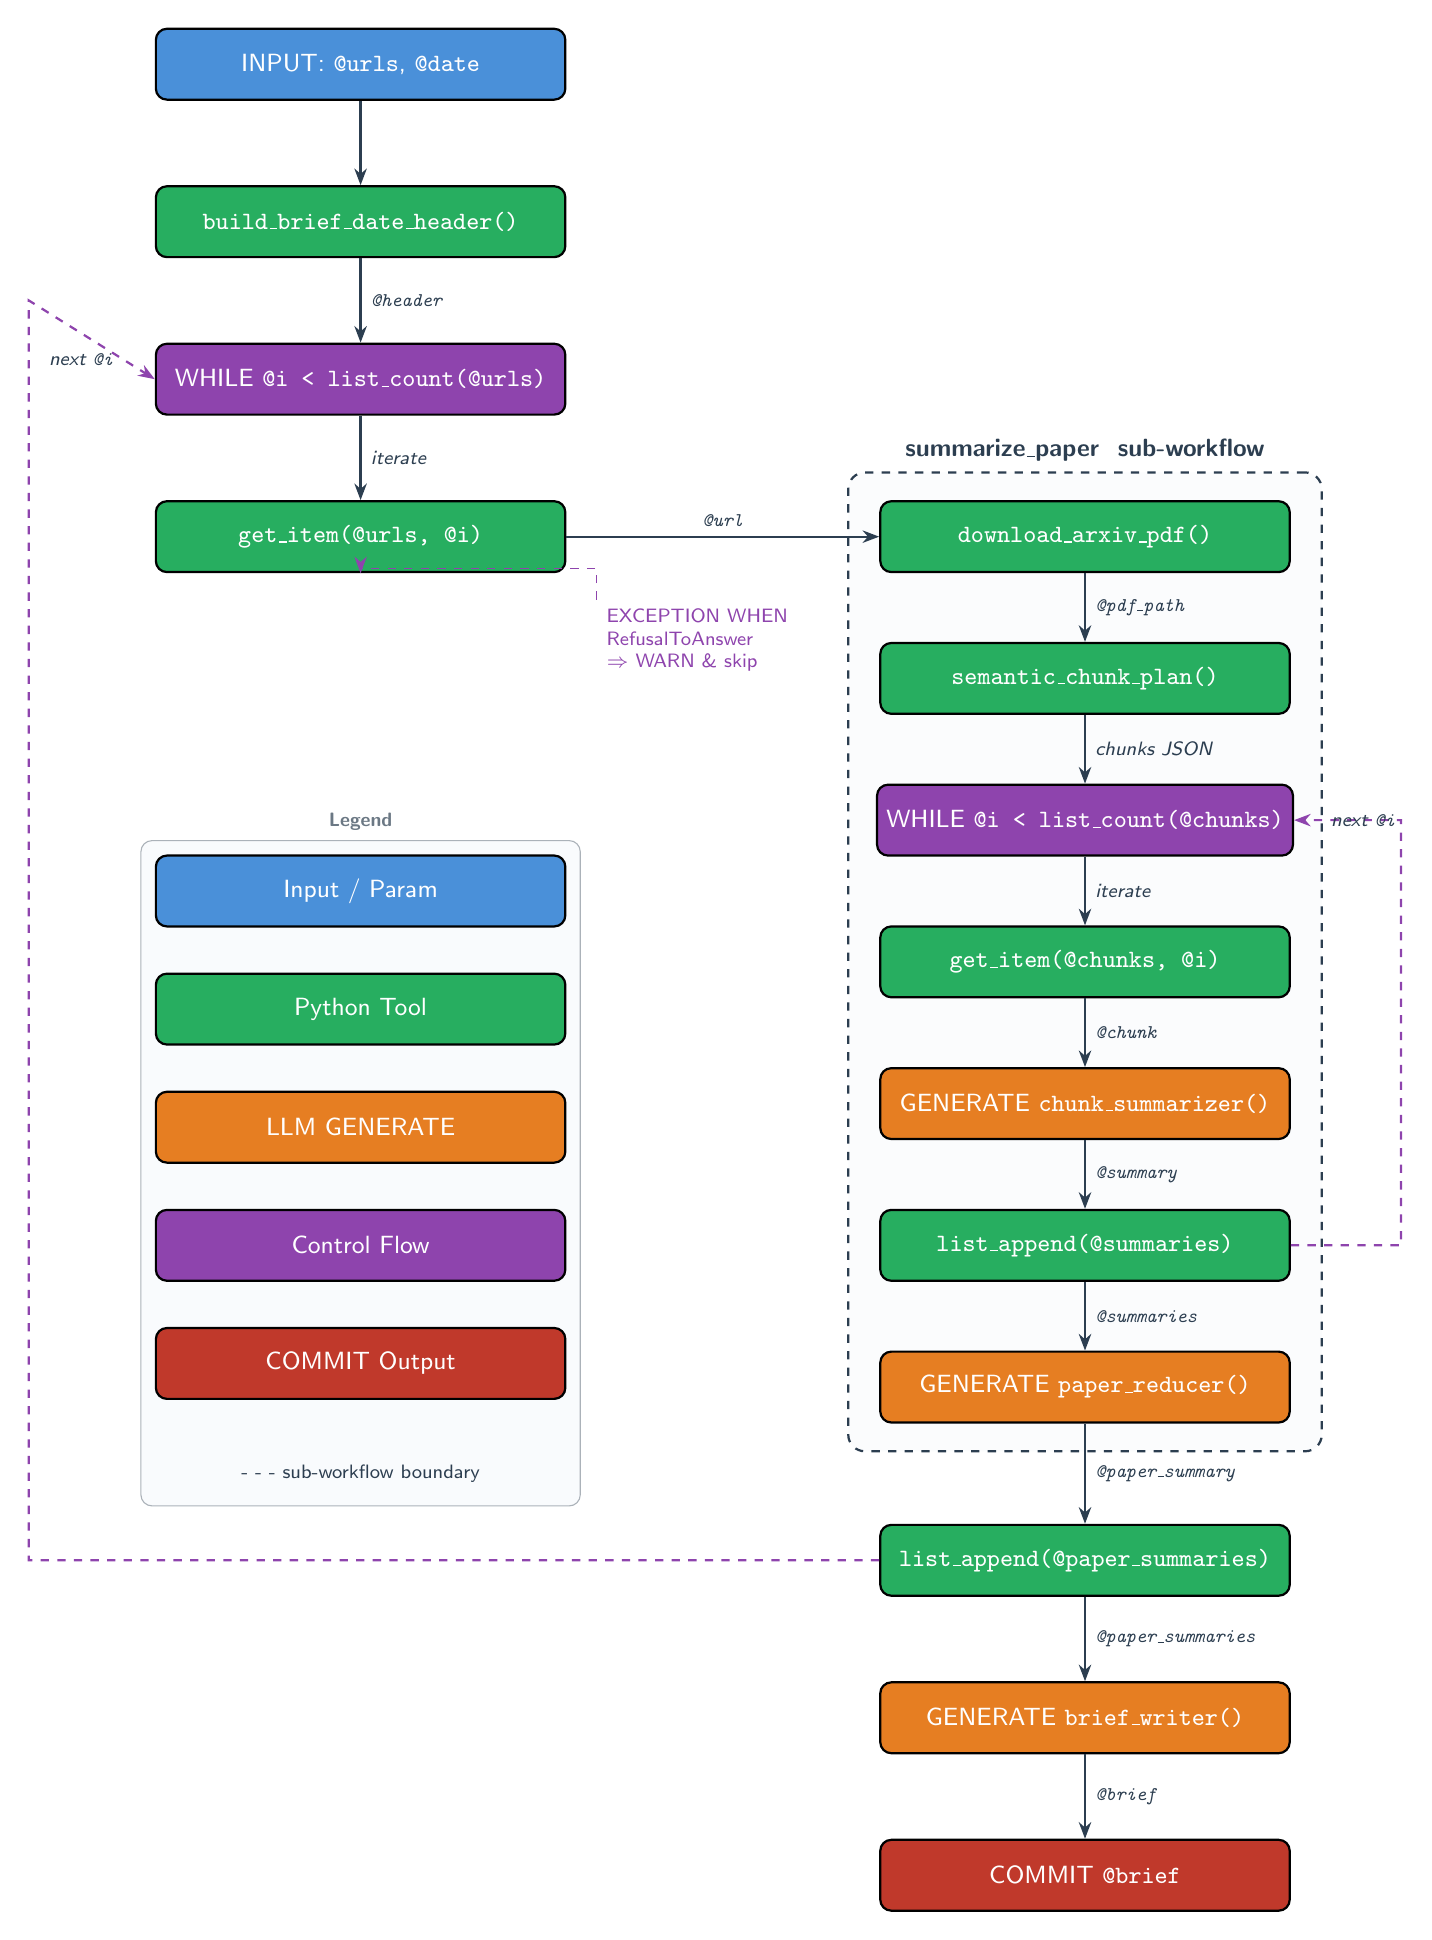
\begin{tikzpicture}

% ══════════════════════════════════════════════════════════════════════════
%  LEFT COLUMN — orchestrator (top nodes only)
% ══════════════════════════════════════════════════════════════════════════

\node[input]  (inp)  at (0,    0  ) {INPUT: \texttt{@urls},  \texttt{@date}};
\node[tool]   (hdr)  at (0,   -2.0) {\texttt{build\_brief\_date\_header()}};
\node[ctrl]   (wurl) at (0,   -4.0) {WHILE \texttt{@i < list\_count(@urls)}};
\node[tool]   (gurl) at (0,   -6.0) {\texttt{get\_item(@urls, @i)}};

% ══════════════════════════════════════════════════════════════════════════
%  RIGHT COLUMN — sub-workflow + orchestrator tail
%  Spacing: 1.8 between sub-workflow nodes, same 2.0 for tail
% ══════════════════════════════════════════════════════════════════════════

\node[tool]   (dl)    at (9.2,  -6.0 ) {\texttt{download\_arxiv\_pdf()}};
\node[tool]   (chk)   at (9.2,  -7.8 ) {\texttt{semantic\_chunk\_plan()}};
\node[ctrl]   (wchk)  at (9.2,  -9.6 ) {WHILE \texttt{@i < list\_count(@chunks)}};
\node[tool]   (gchk)  at (9.2, -11.4 ) {\texttt{get\_item(@chunks, @i)}};
\node[llm]    (csum)  at (9.2, -13.2 ) {GENERATE \texttt{chunk\_summarizer()}};
\node[tool]   (ladd2) at (9.2, -15.0 ) {\texttt{list\_append(@summaries)}};
\node[llm]    (red)   at (9.2, -16.8 ) {GENERATE \texttt{paper\_reducer()}};

% ── Sub-workflow panel ──────────────────────────────────────────────────
\begin{scope}[on background layer]
  \node[panel,
        fit=(dl)(chk)(wchk)(gchk)(csum)(ladd2)(red),
        label={[font=\sffamily\bfseries\small, color=clrSub]above:
               \textit{summarize\_paper}~~sub-workflow}] (swpanel) {};
\end{scope}

% ── Orchestrator tail (below sub-workflow, right column) ─────────────────
\node[tool]   (ladd) at (9.2, -19.0 ) {\texttt{list\_append(@paper\_summaries)}};
\node[llm]    (bwrt) at (9.2, -21.0 ) {GENERATE \texttt{brief\_writer()}};
\node[output] (cmt)  at (9.2, -23.0 ) {COMMIT \texttt{@brief}};

% ══════════════════════════════════════════════════════════════════════════
%  Arrows — orchestrator
% ══════════════════════════════════════════════════════════════════════════

\draw[arr] (inp)  -- (hdr);
\draw[arr] (hdr)  -- (wurl) node[lbl, right]{\texttt{@header}};
\draw[arr] (wurl) -- (gurl) node[lbl, right]{iterate};

% CALL — horizontal dispatch into sub-workflow (same y)
\draw[arr] (gurl.east) -- (dl.west)
           node[lbl, above]{\texttt{@url}};

% red → ladd: vertical, with a small gap across the panel border
\draw[arr] (red.south) -- (ladd.north)
           node[lbl, right]{\texttt{@paper\_summary}};

\draw[arr] (ladd) -- (bwrt) node[lbl, right]{\texttt{@paper\_summaries}};
\draw[arr] (bwrt) -- (cmt)  node[lbl, right]{\texttt{@brief}};

% WHILE @urls back-edge:  ladd → bottom-left route → wurl.west
% path: ladd.west → go left across to x=-1.6 → up to y=-4 → wurl.west
\draw[rarr]
  (ladd.west)
    -- ++(-10.8, 0)                     % go left to x = 9.2-10.8 = -1.6
    -- ++(0,     16.0)                  % go up from y=-19 to y=-3 (≈wurl.north)
    -- (wurl.west)
  node[lbl, near end, left]{next \texttt{@i}};

% ══════════════════════════════════════════════════════════════════════════
%  Arrows — sub-workflow internals
% ══════════════════════════════════════════════════════════════════════════

\draw[arr] (dl)    -- (chk)   node[lbl, right]{\texttt{@pdf\_path}};
\draw[arr] (chk)   -- (wchk)  node[lbl, right]{chunks JSON};
\draw[arr] (wchk)  -- (gchk)  node[lbl, right]{iterate};
\draw[arr] (gchk)  -- (csum)  node[lbl, right]{\texttt{@chunk}};
\draw[arr] (csum)  -- (ladd2) node[lbl, right]{\texttt{@summary}};
\draw[arr] (ladd2) -- (red)   node[lbl, right]{\texttt{@summaries}};

% WHILE @chunks back-edge — right side of sub-workflow column
\draw[rarr]
  (ladd2.east) -- ++(1.4, 0)
               -- ++(0,   5.4)
               -- (wchk.east)
  node[lbl, near end, right]{next \texttt{@i}};

% ══════════════════════════════════════════════════════════════════════════
%  Exception annotation
% ══════════════════════════════════════════════════════════════════════════

\node[font=\sffamily\scriptsize, text=clrCtrl,
      align=left, anchor=north west]
  (exc) at (3.0, -6.8)
  {EXCEPTION WHEN\\RefusalToAnswer\\$\Rightarrow$ WARN \& skip};
\draw[rarr, thin] (exc.north west) -- ++(0, 0.4) -| (gurl.south);

% ══════════════════════════════════════════════════════════════════════════
%  Legend — lower left, single vertical column
% ══════════════════════════════════════════════════════════════════════════

\node[legbox, input]  (l1) at (0, -10.5) {Input / Param};
\node[legbox, tool]   (l2) at (0, -12.0) {Python Tool};
\node[legbox, llm]    (l3) at (0, -13.5) {LLM GENERATE};
\node[legbox, ctrl]   (l4) at (0, -15.0) {Control Flow};
\node[legbox, output] (l5) at (0, -16.5) {COMMIT Output};
\node[font=\sffamily\scriptsize, text=clrSub,
      align=center, minimum width=15mm]
  (l6) at (0, -17.9) {- - - sub-workflow boundary};

% legend frame
\begin{scope}[on background layer]
  \node[draw=clrSub!40, rounded corners=4pt,
        fill=clrBg, fill opacity=0.7,
        inner sep=5pt,
        fit=(l1)(l2)(l3)(l4)(l5)(l6),
        label={[font=\sffamily\bfseries\scriptsize,
                color=clrSub!70]above:Legend}] {};
\end{scope}

\end{tikzpicture}
\end{document}
